\srsfuncion{Introducir plan de vuelo}
	Esta función debe añadir un nuevo vuelo a la lista de vuelos de la compañía aérea.

	\begin{enumerate}
		\item \textit{Entradas}
			\begin{enumerate}
				\item Los campos a introducir por el usuario son: \gls{numero_de_vuelo}, fecha y hora de origen y llegada, aeropuerto de origen y destino, el modelo de avión y el  precio total según la clase (turista, turista superior, business y primera) y tipo de pasajero (adulto, niño y bebé).
				\item El número de vuelo caracteriza e identifica unívocamente a todos los vuelos operados por la compañía. Si dicho parámetro es introducido, todos los demás deben ser ignorados en la búsqueda. Se ha de comprobar que el formato del número de vuelo se corresponde con una sucesión de 4 carácteres numéricos (si el número de caracteres es menor que 4 se completará con \verb|0| por la izquierda).
				\item No se debe permitir introducir fechas u horas no válidas.
				\item Los aeropuertos de origen y destino son un conjunto finito y han de haber sido configurados previamente. Internamente se componen de nombre, ciudad y código \gls{IATA}; externamente se visualizan como una secuencia de texto configurada. El usuario podrá seleccionar uno entre ellos para cada entrada (operación que se puede abreviar introduciendo el código IATA).
				\item El modelo de avión tiene que estar disponible en las fechas indicadas, así como en un correcto estado para su funcionamiento. Por supuesto, dicho modelo debe estar registrado en el inventario.
			\end{enumerate}
		\item \textit{Flujo de operaciones}
			\begin{enumerate}
				\item Se muestra un formulario con los campos anteriormente descritos.
				\item El usuario completa obligatoriamente todos los campos. Ningún campo permite entradas erróneas por definición, salvo el de código de aeropuertos, que tras introducir un código de aeropuerto válido lo selecciona en el \gls{combobox} de aeropuertos y si no es válido no tiene efecto alguno, restaurándose su valor original.
				\item Para cada tipo de clase y de pasajero se mostrará un botón \verb|Calcular precio| que permitirá determinar el precio del vuelo en función del pasajero.
				\item Se crea el nuevo vuelo pulsando sobre el botón \verb|Añadir vuelo|.
			\end{enumerate}
		\item \textit{Respuesta a situaciones no previstas}
			\begin{enumerate}
				\item Si no se puede acceder a la base de datos de configuraciones: no mostrar la pantalla de inicio de la función e informar del error al usuario.
				\item Si alguno de los datos es erróneo: informar al usuario y volver a solicitar la información.
			\end{enumerate}
	\end{enumerate}
	\begin{figure}[ht]\centering
	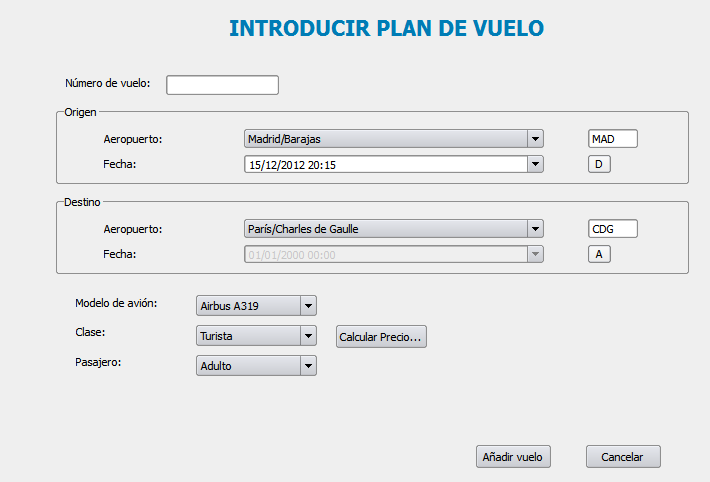
\includegraphics[scale=.6]{imagenes/introducirPlanDeVueloImagen.png}
	\caption{Pantalla aproximada de como introducir un nuevo vuelo}
\end{figure}
